\chapter{Sistema Proposto} \label{cap3}

Neste capítulo é abordado o sistema de detecção de $f_0$ proposto neste projeto, com a descrição da metodologia e dos materiais utilizados no desenvolvimento.

\section{Visão geral}

O sistema proposto é composto pelo bloco de detecção de $f_0$ envolto no ambiente de experimentação, desenvolvido com a finalidade de facilitar a análise de um arquivo de áudio, de modo que tal tarefa possa ser executada apenas por meio de uma interface gráfica. A Figura \ref{fig-system-1} mostra uma visão geral do projeto. Dado um arquivo de áudio como entrada, o bloco de pré-processamento é responsável pelo preparo da mídia para a análise, definindo o tamanho da janela a ser analisada e executando qualquer processamento que seja necessário para que a detecção seja feita. Após isso, o áudio é submetido ao bloco de detecção de $f_0$, que fará a detecção para cada deslocamento da janela de tempo. Por fim, a saída do bloco de detecção de $f_0$ é plotada na janela principal da aplicação, de modo a ser comparada visualmente com os registros originais de notas e tempo do áudio. 

\begin{figure}[h]
	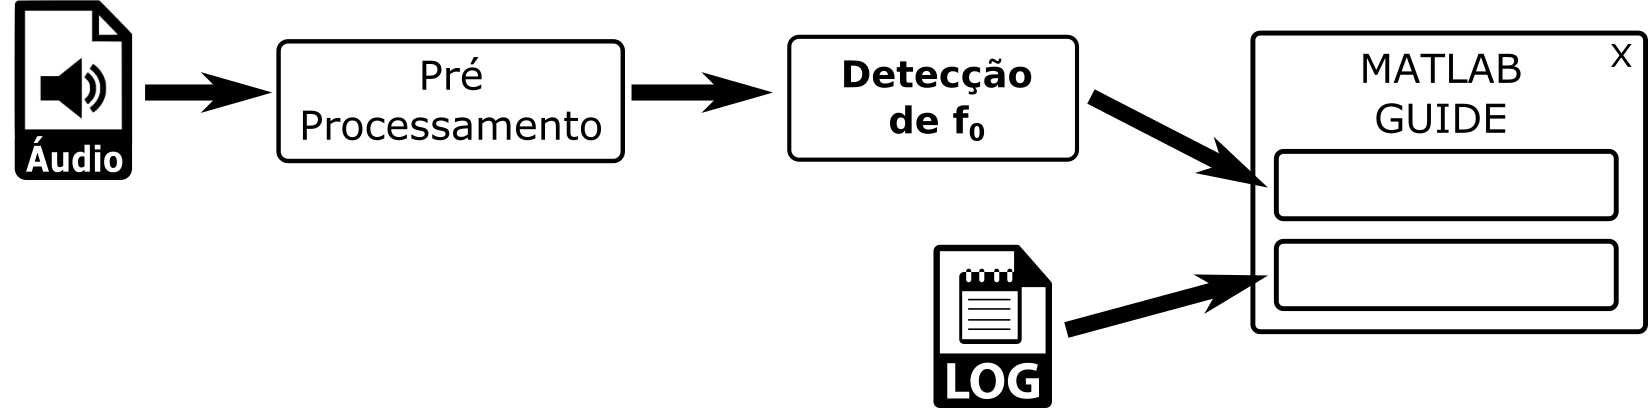
\includegraphics[width=\linewidth]{pasta1_figuras/system1c.png}
	\caption{Estrutura do sistema desenvolvido}
	\label{fig-system-1}
\end{figure}

O sistema foi desenvolvido em linguagem MATLAB\rreg, utilizando a ferramenta de interface gráfica GUIDE para interação com o usuário, fornecendo a lista de áudios disponíveis na base de dados para a execução do algoritmo de detecção e retornando, ao término da execução, os gráficos necessários para a análise visual do áudio. Os registros originais de notas e tempo dos áudios estão em formato texto, em arquivos com extensão $.log$. Os áudios de entrada devem estar em formato reconhecido pelo MATLAB\rreg. Para a execução de um experimento, um usuário precisará fornecer o áudio, seu respectivo arquivo de registros de tempo de notas, a velocidade da música, em batidas por minutos, e a referência de menor nota para a detecção, que é um valor referente a menor nota executada no áudio a ser analizado.

\section{Bloco de Pré-Processamento}

O bloco de pré-processamento é responsável pelo preparo do áudio para a detecção de $f_0$. Esse bloco recebe como entrada o caminho para o arquivo de áudio, seu valor de batidas por minutos (bpm) e um número real positivo equivalente a nota de menor tempo de duração desejada na detecção. O diagrama da figura \ref{flowchart-preprocessing} demonstra o funcionamento dessa parte inicial do sistema. Primeiro, lê-se o arquivo de áudio a partir do caminho fornecido. Para isso, a função \textit{audioread}, nativa do MATLAB\rreg, foi utilizada e retorna as amostras do áudio e sua $f_s$. Após, obtém-se as informações de metadados presentes no arquivo. A função \textit{audioinfo}, também nativa da linguagem utilizada, busca as informações do áudio como duração e número de canais. 

\begin{figure}[h]
	\centering
	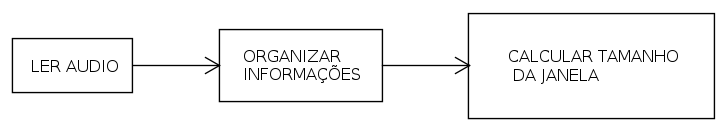
\includegraphics[width=\linewidth]{pasta1_figuras/preprocessing.png}
	\caption{Diagrama do bloco de pré-processamento}
	\label{flowchart-preprocessing}
\end{figure}

Após a leitura do áudio e de suas informações, o sistema determina o tamanho da janela para análise de tempo curto. Tal comprimento de janela não pode ser muito pequeno, ao ponto de não ter amostras suficientes para análise, e também não pode ser tão grande, para não misturar em uma mesma posição de janela um intervalo com duas $f_0$ diferentes. Deste modo, optou-se por um tamanho em que a duração do intervalo não fosse maior do que o tempo de referência de nota mínima. Utilizando essa referência, é possível garantir que o sistema não fará análise de uma janela com duas $f_0$'s. Essa entrada é dada em função da velocidade de execução da música (em $bpm$), sendo que uma nota mínima de referência $1$ equivale a uma nota por batida. Para definir o tamanho da janela em quantidade de amostras, foi utilizado:

\begin{enumerate}
	\item Converter o valor de $bpm$ para batidas por segundos, multiplicando por 60;
	\item Dividir o valor de duração da menor nota por dois, de modo a analisar 2 vezes a menor nota;
	\item Multiplicar batidas por segundos por metade da menor nota e a frequência de amostragem, obtendo a quantidade de amostras em uma janela
\end{enumerate}

Os pontos acima são expressos na equação (\ref{eq-windowSizeExp}):

\begin{equation}
L = \frac{60}{bpm}\frac{t_{ref}}{2}F_s
\label{eq-windowSizeExp}
\end{equation}

onde $t_{ref}$ é o tempo de referência de duração da menor nota a ser detectada e $bpm$ é a velocidade de execução da música no áudio, em batidas por minutos. 


Simplificando, obtém-se a equação (\ref{eq-windowSize}):

\begin{equation}
	L = \frac{30t_{ref} F_s}{bpm}
	\label{eq-windowSize}
\end{equation}

Em linha de código, foi necessário ainda arredondar o valor de $L$, visto que posições de amostras devem ser valores inteiros. Para isso, utilizou-se a função nativa \textit{round} do MATLAB\rreg.


Com o tamanho da janela definido, o áudio segue para o bloco de detecção de $f_0$.

\section{Bloco de Detecção de $f_0$}

A detecção de $f_0$ é feita através da STFT, utilizando a FFT. O método de detecção consiste em transportar a janela sob análise do áudio para o domínio da frequência, de modo que seja possível localizar a frequência de maior amplitude nessa janela. Essa frequência é registrada como a $f_0$ do respectivo intervalo. O tamanho do deslocamento da janela é igual ao comprimento da mesma, de modo que não se repitam amostras entre um deslocamento e outro. Outros métodos de deslocamento podem ser adotados de acordo com o tipo de problema que deseja-se solucionar, por exemplo, para a detecção exata do tempo de início das notas, um deslocamento menor que o tamanho da janela permitiria verificar com mais precisão o ponto de início de cada nota. O algoritmo desse bloco pode ser dividido em três partes: A pré-análise, o deslocamento da janela e a análise de detecção de $f_0$. Após esses passos, o bloco retorna a $f_0$ detectada.


A parte de pré-análise consiste basicamente na inicialização das variáveis que serão utilizadas no momento da análise. A função \textit{zeros}, nativa do MATLAB\rreg, é utilizada para gerar vetores de zeros do tamanho esperado para a saída da detecção. Para o tamanho de janela igual ao deslocamento, o comprimento da saída pode ser calculado pela divisão do tamanho total do áudio pelo comprimento da janela. Durante a execução do código, o vetor de saída, inicialmente preenchido com zeros, receberá cada uma das detecções, e será retornado finalmente com todas as frequências fundamentais obtidas em cada posição da janela.


Na parte de deslocamento da janela, um laço é utilizado, conforme o diagrama da Figura \ref{flowchart-deslocamento}. A variável \textit{CONTADOR} é utilizada para marcar o posicionamento das saídas das detecções, sendo incrementado a cada execução do laço, enquanto o iterador \textit{i} do laço é usado para marcar a posição da janela sobre o áudio. O tamanho do deslocamento da janela é definido como a variável \textit{windowSize}, que é o comprimento dessa janela, de modo a garantir que cada amostra será analizada apenas uma vez. A parte do áudio no intervalo do deslocamento da janela é retirado para a variável \textit{window}, esse será o sinal analizado. A análise é invocada com \textit{DETECTAR\_F0(window)}, que é a função desenvolvida para a detecção das frequências fundamentais, retornando para cada janela uma $f_0$ detectada. Por fim, essa frequência retornada é armazenada no vetor de saída, conforme a posição guardada na variável \textit{CONTADOR}, e se repete todo o procedimento até que a janela tenha se deslocado por todo o áudio.

\begin{figure}[h!]
	\centering
	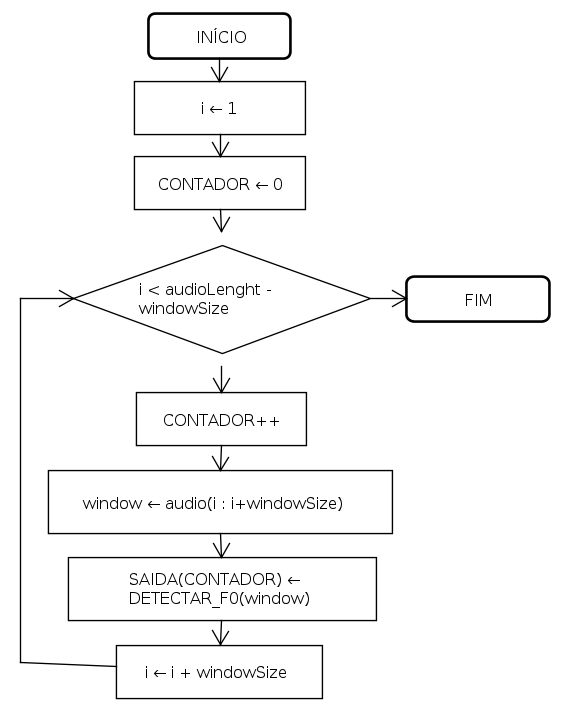
\includegraphics[scale=1]{pasta1_figuras/deslocamento.png}
	\caption{Diagrama do algorítmo de deslocamento da janela}
	\label{flowchart-deslocamento}
\end{figure}

A terceira e última parte do bloco de detecção de $f_0$ é o método responsável pela execução da FFT e identificação da fundamental. A função foi desenvolvida tendo como base as aplicações exemplo da \textit{fft} do MATLAB\rreg, de modo que todo o tratamento pós-transformada é feito conforme as recomendações obtidas na documentação. A implementação adotada é capaz de fazer a detecção da $f_0$ em um tempo consideravelmente rápido, de modo que a janela possa ser deslocada rapidamente e, consequentemente, finalizar a análise do áudio em poucos segundos. O redimensionamento da quantidade de amostras a serem transformadas também cooperou para a boa performance do código.


A função, exibida no Algorítmo \ref{analyse}, recebe como entrada a janela de áudio, na variável $x(t)$, e a frequência de amostragem. Sua saída é a $f_0$ detectada. Da linha 2 à 5, o sinal sob análise é preenchido com \textit{padding} de zeros de modo a satisfazer o tamanho de $2^{16}$ amostras. Como visto na fundamentação teórica, este passo é importante para a performance do algoritmo. Na linha 6, a FFT do MATLAB\rreg é executada, transportando a janela de áudio para o domínio da frequência. É importante ressaltar que a saída da FFT tem o mesmo comprimento que a entrada. Uma das características da FFT está em que sua saída é multiplicada pela quantidade de amostras. Desse modo, na linha 7, foi necessário dividir pelo comprimento da janela ao fim da transformação. Na mesma linha também calcula-se o módulo do sinal complexo. Na linha 8, devido ao espelhamento na frequência, retira-se metade do vetor do espectro e, na linha 9, dobram-se as amplitudes como tratamento padrão para os efeitos da transformação pela FFT. Após todos esses passos, as linhas de 11 à 13 identificam a frequência fundamental da janela sob análise buscando a frequência com amplitude máxima do vetor do espectro.
\\
\begin{algorithm}
	\caption{Função de detecção de $f_0$}
	\label{analyse}
	\begin{algorithmic}[1]
		\Function{DETECTAR\_F0}{$x(t)$, $f_s$}
			\State $\Delta$ = $COMPRIMENTO(sinal)$
			\State $\Delta_{ideal}$ = $2^{16}$;
			\State $x(t)$ = $CONCATENA(x(t), zeros(\Delta_{ideal}- \Delta))$
			\State $\Delta$ = $\Delta_{ideal}$
			\State $X(w)$ = $FFT(x(t))$
			\State $P2$ = $ABSOLUTO(X(w)/\Delta)$
			\State $P1$ = $P2(1:\frac{\Delta}{2} + 1)$
			\State $P1(2:fim-1)$ = $2 * P1(2:fim-1)$
			\State $f$ = $f_s$ * $(0 : \frac{\Delta}{2})/\Delta$
			\State $A_{max} = MAX(P1(:))$
			\State $i_{max}$ = $POSI\c{C}\tilde{A}O(A_{max}, P1)$
			\State $f_0$ = $f(i_{max})$
			\State \Return $f_0$
		\EndFunction
	\end{algorithmic}
\end{algorithm}

Conforme visto no diagrama da Figura \ref{flowchart-deslocamento}, o retorno da função de detecção de $f_0$ é armazenado em um vetor de saída do bloco, que será fornecido à interface GUIDE para a plotagem do gráfico dos resultados da detecção em cada deslocamento da janela.


\section{Interface GUIDE}

Com o propósito de facilitar o uso do sistema, foi desenvolvida, através da ferramenta GUIDE\cite{mathworks2018guide} do MATLAB\rreg, uma interface gráfica para o usuário, que é exibida na Figura \ref{fig-guide-1}. Na janela, é disponibilizado ao usuário um menu $popup$ com a lista dos áudios disponíveis no diretório do projeto e um botão \textit{PLAY}. Ao selecionar um arquivo e executar, a interface inicia o algoritmo de detecção de pitch com os parâmetros necessários para a análise. Janelas desenvolvidas em GUIDE utilizam \textit{callbacks} para seus componentes, de modo que a chamada para a detecção está na \textit{callback} do botão. A interface foi desenvolvida com o objetivo de ser utilizada para testes de algoritmos de detecção de $f_0$ e \textit{pitches}, de modo que é possível incorporar outros algoritmos sempre que necessário, e de maneira rápida.


Ao término da detecção, são exibidas na interface 4 gráficos: (i) O sinal de áudio no tempo, que permite ter noção da localização das notas e de cada trecho de uma música, (ii) o espectrograma do áudio, que permite uma localização visual das frequências fundamentais, (iii) as saídas do sistema de detecção de pitch no tempo, saída a ser analisada e comparada com o espectrograma e os registros, e (iv) as saídas do sistema de detecção de pitch no tempo sobrepostas nas saídas esperadas, obtidas do arquivo de registro original de notas e tempos do áudio. O último gráfico permite que se faça uma avaliação visual rápida sobre as detecções, sendo possível identificar os trechos onde o sistema encontrou maiores dificuldades de detectar a $f_0$.

\begin{figure}[h!]
	\begin{subfigure}{1\textwidth}
			\centering
			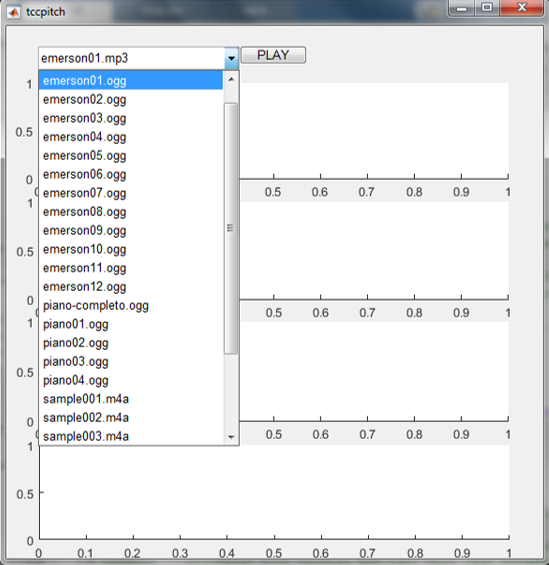
\includegraphics[scale=0.6]{pasta1_figuras/guide1.png}
	\end{subfigure}
	\hspace*{\fill} % separation between the subfigures
	\begin{subfigure}{1\textwidth}
		\centering
		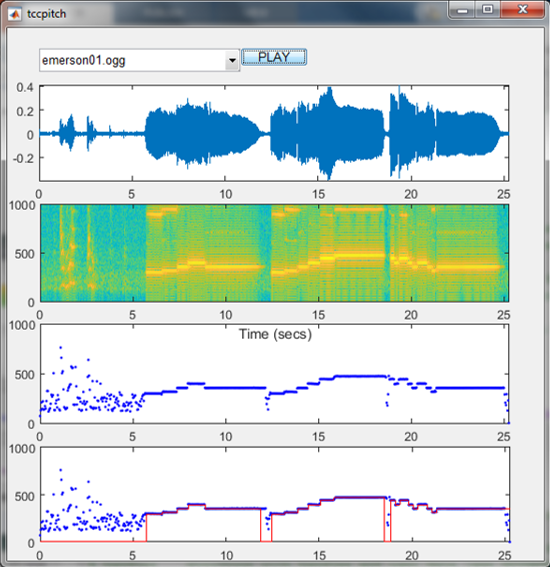
\includegraphics[scale=0.6]{pasta1_figuras/guide2.png}
	\end{subfigure}
	\caption{Interface GUIDE}
	\label{fig-guide-1}
\end{figure}

O projeto foi organizado de modo que a aplicação é lançada a partir do arquivo GUIDE. Demais funções estão disponíveis no mesmo diretório, em arquivos com extensão $.m$, sendo chamadas pela interface quando necessário. Os arquivos da base de dados (Áudios e registros de logs) são armazenas em subdiretórios específicos para cada tipo: Os áudios ficam no subdiretório \textit{samples}, enquanto os registros ficam no subdiretório \textit{logs}. O menu \textit{popup} com a lista de áudios da base de dados é criado por meio da \textit{callback} de criação do próprio menu, que é chamada pela interface logo na inicialização. Para o preenchimento da lista desse menu, obtém-se a lista de áudios do subdiretório \textit{``samples''} por meio da função \textit{``getFiles''}, que mapeia o diretório e retorna uma lista com todos os arquivos internos no subdiretório.


Os gráficos foram gerados de modo nativo pelo matlab, através da função \textit{plot}, com exceção do espectrograma que possui função específica para isso. Após a geração dos gráficos, todos foram setados na mesma escala, de modo a exibir o áudio completo e as frequências máximas detectadas. Verificou-se que, em alguns casos, o espectrograma não aparece por completo, devido ao seu tamanho limitado. Para melhor visualização de todos os gráficos, também é possível plota-los de maneira isolada da janela, através do comando \textit{figure}, nativo do MATLAB\rreg.


% Tentar explicar cada um dos componentes da janela (dropdown, gráficos, botões)

\section{Construção da Base de Dados}

A base de dados construída para este projeto consiste em dois diretórios, onde um contém os arquivos de áudio para experimentos e o outro contém os registros de tempos de notas para os áudios. Foram feitas gravações com os instrumentos sax alto, clarinete, piano eletrônico e violão acústico. Ao término do projeto, a base foi disponibilizada de modo público por meio de um repositório GIT\cite{cruzjr2018}.


As gravações dos áudios da base de dados foram feitas com um \textit{smartphone}. Foi utilizado a aplicação de gravador do sistema Android\rreg, que já conta com uma filtragem básica. As gravações foram realizadas em ambientes de pouco ruído, de modo a se obter um áudio com uma qualidade mínima necessária para a identificação das notas. Cada instrumento foi gravado pelo menos 3 vezes, executando 2 músicas em diferentes velocidades e, por fim, executando uma escala maior com velocidade de 2 tempos para cada nota. O violão e o piano executaram uma escala maior em Dó (C), enquanto o sax alto executou em Mi Bemol (Eb), e o clarinete em Si Bemol(Bb). Isto ocorreu devido às próprias características desses instrumentos, que possuem afinação em tons diferentes.

\begin{table}[h!]
	\centering
	\caption{Lista de Gravações da Base de Dados} 	\label{table-songs}
	\begin{tabular}{|c|c|}
		\hline
		\textbf{INSTRUMENTO}       & \textbf{ÁUDIO}             \\ \hline
		\multirow{3}{*}{CLARINETE} & Escala - Bb Maior         \\ \cline{2-2} 
		& Música - \textit{Agnus Dei}         \\ \cline{2-2} 
		& Música - Super Mário Brós  \\ \hline
		\multirow{3}{*}{SAX ALTO}  & Escala - Eb Maior           \\ \cline{2-2} 
		& Música - Deus Cuida de Mim \\ \cline{2-2} 
		& Música - \textit{Summertime}        \\ \hline
		\multirow{3}{*}{PIANO ELETRÔNICO}     & Escala - C Maior           \\ \cline{2-2} 
		& Música - Eu Navegarei      \\ \cline{2-2} 
		& Música - \textit{Skyfall}         \\ \hline
		\multirow{3}{*}{VIOLÃO}    & Escala - C Maior           \\ \cline{2-2} 
		& Música - Nona Sinfonia     \\ \cline{2-2} 
		& Música - Ao Deus de Abraão \\ \hline
	\end{tabular}
\end{table}

Após as gravações, foram selecionados 2 áudios de música e o áudio da escala maior de cada instrumento, os quais foram inseridos no subdiretório \textit{``samples''}, onde reunem-se todos os áudios da base. Todas as músicas gravadas para este projeto foram escolhidas pelos próprios instrumentistas, de modo a popular a base de dados com melodias mais comuns entre eles. Estipulou-se apenas 3 critérios:

\begin{itemize}
	\item Tocar apenas a melodia, sem acompanhamento;
	\item Tocar apenas uma nota por vez, sem notas simultâneas;
	\item Duração entre 10 e 25 segundos;
\end{itemize}


A Tabela \ref{table-songs} lista as músicas que foram gravadas para a construção da base de dados.



% de que forma os rquivos foram produzidos
Foi realizado um mapeamento manual dos áudios com o auxílio do software Audacity\cite{audacity2018}, de onde obteve-se informações precisas de tempo e duração de cada nota. Os registros ficam armazenados no subdiretório \textit{``logs''}, e possuem a mesma nomenclatura do respectivo áudio que registram, acrescentados da extensão \textit{``.log''}. Os registros são feitos em formato texto, cada nota soada por linha. Cada linha possui a sigla da respectiva nota, sua frequência fundamental e seu tempo inicial, em segundos, separados por tabulação. Um exemplo do registro é mostrado a seguir:
\\ 
\begin{lstlisting}[
style      = Matlab-editor,
basicstyle = \mlttfamily,
]
XX  0       0
D4  293.66  5.725
D#4 311.13  6.56
F4  349.23  7.4
\end{lstlisting}



No exemplo, pode-se identificar que a primeira nota, um ré na 4ª oitava, é soada no tempo 5.725 segundos. A nota seguinte inicia em 6.56 segundos, um ré sustenido, e por fim, um fá se inicia em 7.4 segundos.

% Fim Capítulo
